\section{Experiments}
\label{experiments}

Closed-loop testing allows us to debug the pacemaker, explore operating conditions, and understand interactions between heart and pacemaker that might lead to undesirable or unsafe behavior.

a) \emph{Debugging the pacemaker}: As an illustration of how a Virtual Heart Model (VHM) can be used to debug a pacemaker, we give a simple example of a pacemaker model in Simulink, connected to a VHM in Simulink as well. 
The pacemaker and VHM models are shown in Fig.~\ref{fig:simulinkModels}.
\begin{figure}[tb]
	\centering
	
\includegraphics[scale=0.2]{placeHolder.pdf}
	\caption{Simulink models of heart and pacemaker.}
	\label{fig:simulinkModels}
\end{figure}
No open-loop testing was conducted on the pacemaker model.
However, 
The requirement given to the tester was that if a PVC or $V_{sense}$ or $V_{pace}$ occur, then the next $V_{pace}$ should not occur before 500ms. 
\todo[inline]{why is this a requirement of good behavior?s}
The specification-guided testing methodology outlined in Section \ref{testingMethodology} quickly found a PVC disturbance waveform that caused the closed loop to violate this specification (fewer than 10 tests).
Debugging revealed that the pacemaker model was missing the behavior that caused it to reset the Upper Rate Interval to its default value after every $V_{sense}$ event.

For the next two experiments, we used a pacemaker model that had been open-loop tested to satisfy a number of specifications from the Boston Scientific Challenge \cite{challenge}.
\todo[inline]{RM: review wording about "leading company"}

b) \todo[inline]{not a good example...}\emph{Manageable heart conditions}: 
The frequency of PVCs has been shown to correlate to some degree with the extent of cardiomyopathy (an anomaly of the heart muscle).
However, there are no definite thresholds for the frequency of PVCs that indicate sure cardiomyopathy, and different authors have used different thresholds that range from 10,000 to 20,000 PVC events per day, or as different percentages of the total beats per day (from 10\% to 24\%) \cite{ChaLKG12_PVC}.

\begin{figure}[tb]
	\centering
	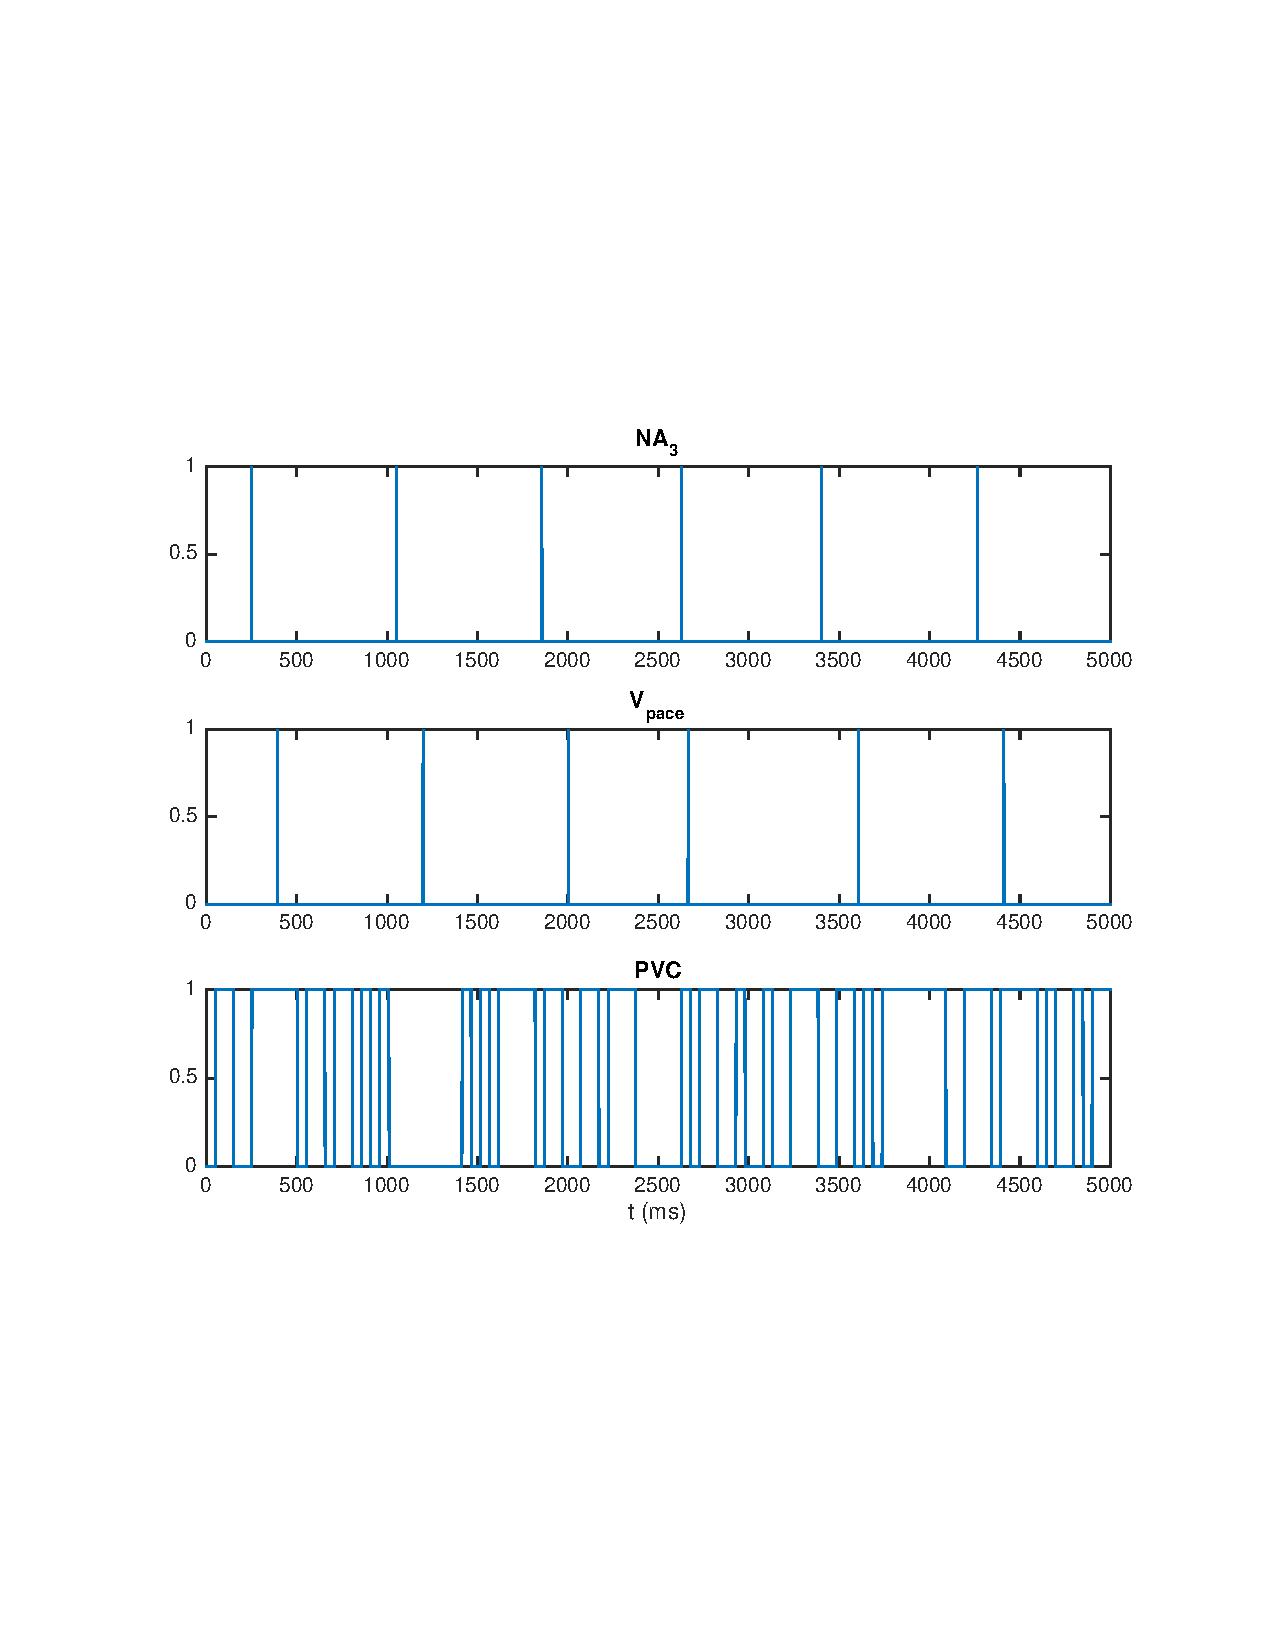
\includegraphics[width=0.7\linewidth]{figures/bug6_kept1.pdf}
	\caption{A high-frequency PVC pattern and associated early ventricular pacing.}
	\label{fig:bug6_kept1}
\end{figure}

% Electrophysiological Characteristics
% PVC Burden
% Several studies have shown that the frequency of PVCs correlates at 
%least modestly with the extent of LV dysfunction and ventricular dilation
%at the time of initial clinical presentation.13?17 Patients with decreased 
%LVEF had a higher mean PVC burden than their counterparts with normal LV 
%function (29%?37% versus 8%?13%).15,18,19 However, there are no clear-cut 
%points that mark the frequency at which cardiomyopathy is unavoidable.
%
%Niwano et al13 used a cut point of 20 000 PVCs over 24 hours to define 
%the high-frequency group, 
% whereas Kanei et al17 used a figure of 10 000 PVCs per day. 
% Other studies defined ?frequent? PVCs as >10% of total beats
%rather than the absolute number of PVCs,18,19 
%
%yet in some cases, a high 
%PVC burden may not impair LV function, whereas PVC-induced cardiomyopathy 
%can be observed in patients with lower PVC frequencies, albeit at lower 
%incidences.12,16,17 
%It is not known why the majority of patients with 
%frequent PVCs have a benign course, whereas up to one third of them 
%develop cardiomyopathy. One possible explanation is that the evaluation 
%of PVC burden using 24-hour Holter monitoring may be inadequate and may 
%misrepresent the patient's true PVC burden.20 
% Baman et al18 suggested that 
%a PVC burden of >24% had a sensitivity and specificity of 79% and 78%, 
%respectively, in separating the patient populations with impaired versus 
%preserved LV function. Nevertheless, the majority of patients presenting 
%with frequent PVCs had preserved LVEF.4,9,12,13,15 Therefore, although 
%significant, the PVC burden is not the only factor contributing to 
%impairment of LV systolic function.9,15,21
% from Advances in Arrhythmia and Electrophysiology. "Premature Ventricular 
% Contraction-Induced Cardiomyopathy A Treatable Condition"
% http://circep.ahajournals.org/content/5/1/229.full 

raised the limit didn't limit the frequency of PVC pulses that can be generated by the tester. 
This allows us to explore how the pacemaker reacts to frequent explored the frequency of PVC impulses be frequent PVC leads to incorrect pacing.

c) \emph{Exploring behavior}: In the third experiment, we set a minimum delay of 400ms between PVC pulses, and tried to falsify the following specification:
``If either Node3 depolarizes or a $V_{pace}$ is issued, a minimum of 500ms must pass before the next $V_{pace}$".
\todo[inline]{why is this a requirement of good behavior?s}
Note that the pacemaker can not distinguish between a $V_{sense}$ caused by a PVC and a $V_{sense}$ caused by path conduction.
\todo[inline]{check last statement}
Thus we need access to the heart model to test this specification, and this can only happen in a closed-loop setting.

The specification was violated by the waveform shown in Fig. \ref{fig:bug8_kept1}.
\begin{figure}[tb]
\centering
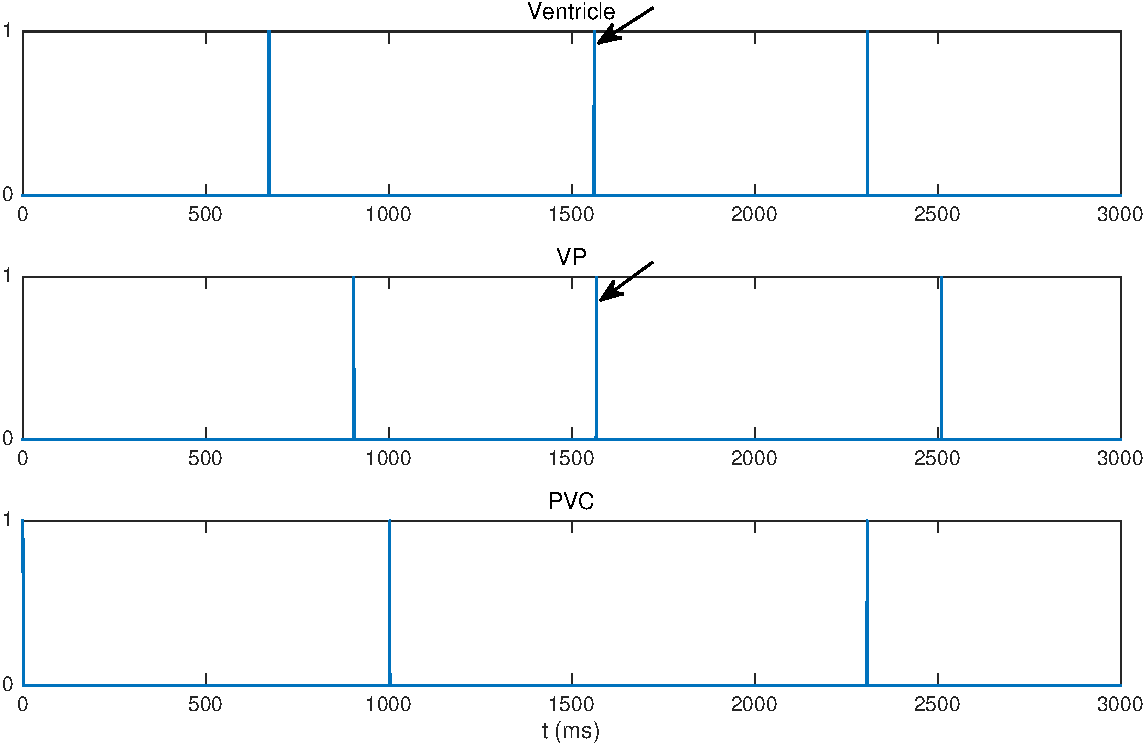
\includegraphics[width=0.7\linewidth]{figures/bug8_kept1}
\caption{A PVC pattern that causes a premature ventricular pacing.}
\label{fig:bug8_kept1}
\end{figure}
Upon investigating the reasons for this violation, it was concluded that the Ventricular Safety Pacing (VSP) feature of our model was at fault: the VSP is a way to prevent the consequences of AV crosstalk, namely, self-inhibition. 
When the pacemaker senses a ventricular event during the VSP interval (but past the PAVB interval), it commits a $V_{pace}$ at the end of the VSP.
In this experiment, a PVC disturbance that occured past the PAVB, but still within the VSP, provoked the ventricular event that led to the early $V_{pace}$.

In this case, the violating trace is due to a desired feature of the pacemaker (preventing self-inhibition).
Thus, the designer and physician must decide whether this is an acceptable case, or whether the pacemaker needs to be adjusted (if at all possible) to prevent this from happening (while maintaining the VSP feature).
